We tried both to always choose
the highest valued action, and selecting an action with probability proportional
to (rescaled) value. This method of breaking ties in the Q matrix proved useful
in board game environments  where the number of states were large, but for the
other environments, it didn't add any benefit and actually caused the agent to
perform worse in some examples. The softer version of choosing proportional to
gain were less successful in all cases. A problem with sticking to the highest
value is that you tend to take one of few extreme paths: in the mines
environment you have a harder time learning to circumventing an obstacle, since
the algorithm causes you to go more in straight lines.

Improvements using tiebreaker?!
Spelar bara roll när man har tie och i små system används den inte ofta. I slutet av runs har man inte ties. En tie är när två Q-värden är samma och vi måste välja en av dom.
Tiebreaker i Connectfour och tic-tac-toe.


When testing our agent on very different environments, from simple board games to context bandit problems. We observe that even very general approaches to improving performance against a large class of environments, might hurt the performance against other environments. We addressed large state space environments, where the state is altered gradually and good actions are good over a range of similar states, and introduced a tie breaker that tries to make informed decisions when faced with a lack of statistical data. This replaced a simple "first best" choice, which turned out to actually be a better decision in some cases. 

We tested two versions of UCB as policies in an attempt to shore up Sarsa($\lambda$)s unsuitability for bandit problems. The idea was to consider all states as independent bandit problems, where the UCB policies would decide the balance between exploration vs exploitation. The simpler UCB1 does not consider any upper bound on the reward and will never be satisfied, this causes it to start exploration even when faced with certain victory options. The KL-UCB considers the case where the reward is bounded. Both however, assumes long time horizons, where exploration occurs gradually. When faced with the short experiments in the competition, where the optimal approach should be to explore first, and exploit in the end

Running the agent with varying step sizes $\alpha$ we observed bad results on all values but $\alpha=1$. Similarly, for most $\lambda$ values...KOLLA HÄR!!

We also noticed that Sarsa($\lambda$) in its original formulation will decide on the next action before it updates the Q matrix. In the specific case where penalties 

Sweep $\lambda$
\begin{figure}[h]
    \centering
    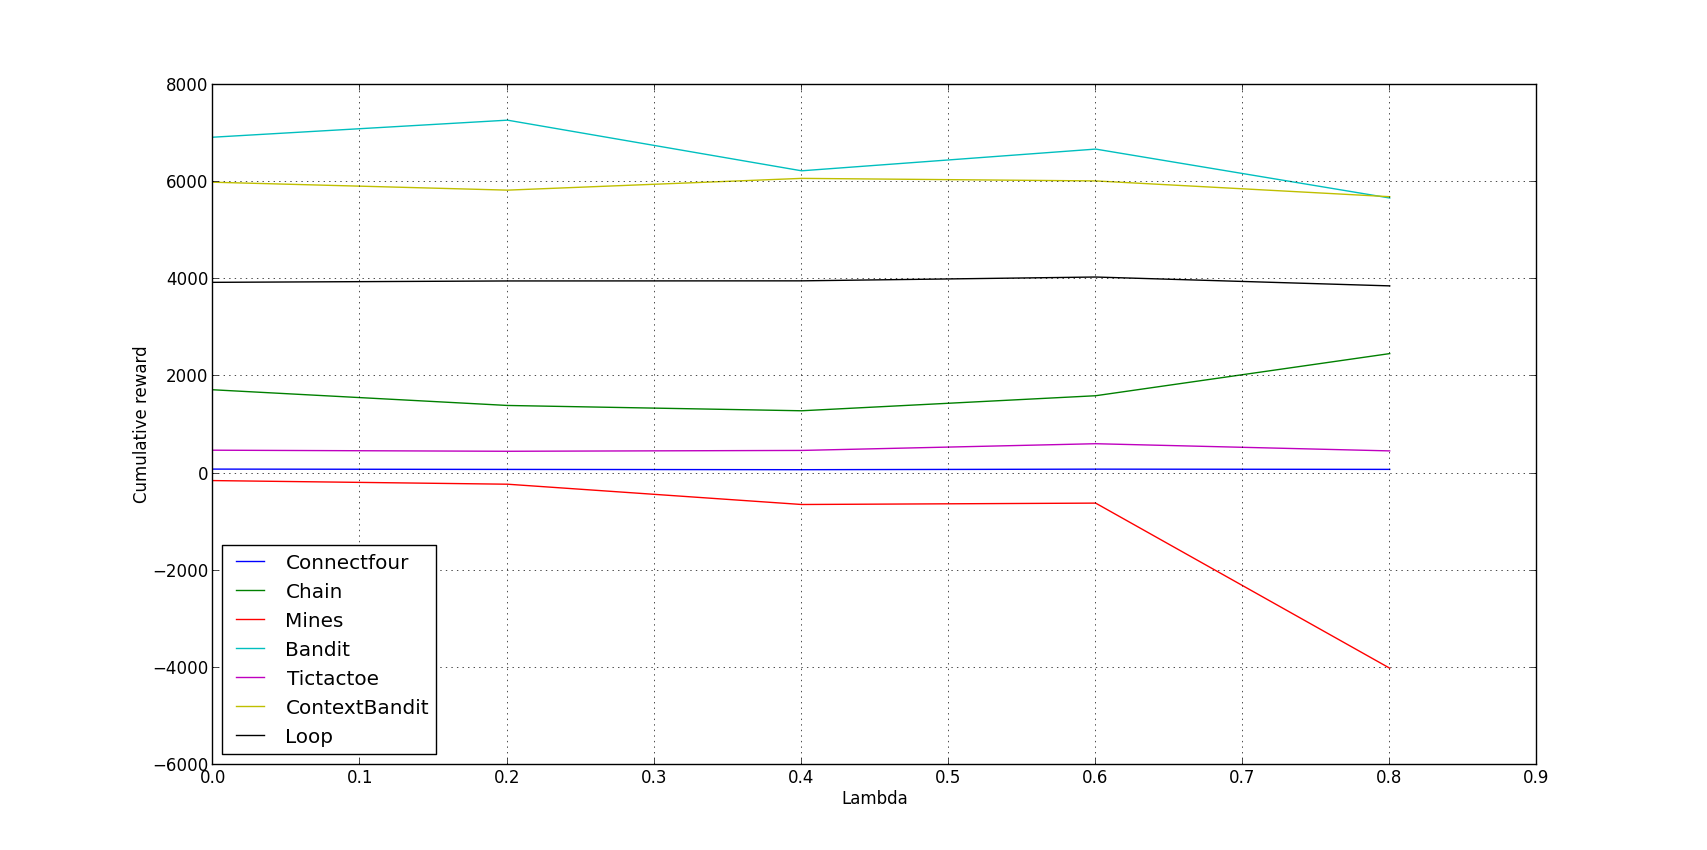
\includegraphics[width=0.5\textwidth]{../data/lambdasweepplot.png}
    \caption{Awesome Image}
    \label{fig:awesome_image}
\end{figure}


Figure~\ref{fig:cumreward} shows how the agents average performance over 50 runs in a 100 episode experiment against all environments with parameters set to $\lambda = 0.2$ and $\alpha = 1$

\begin{figure}[h!]
    \centering
    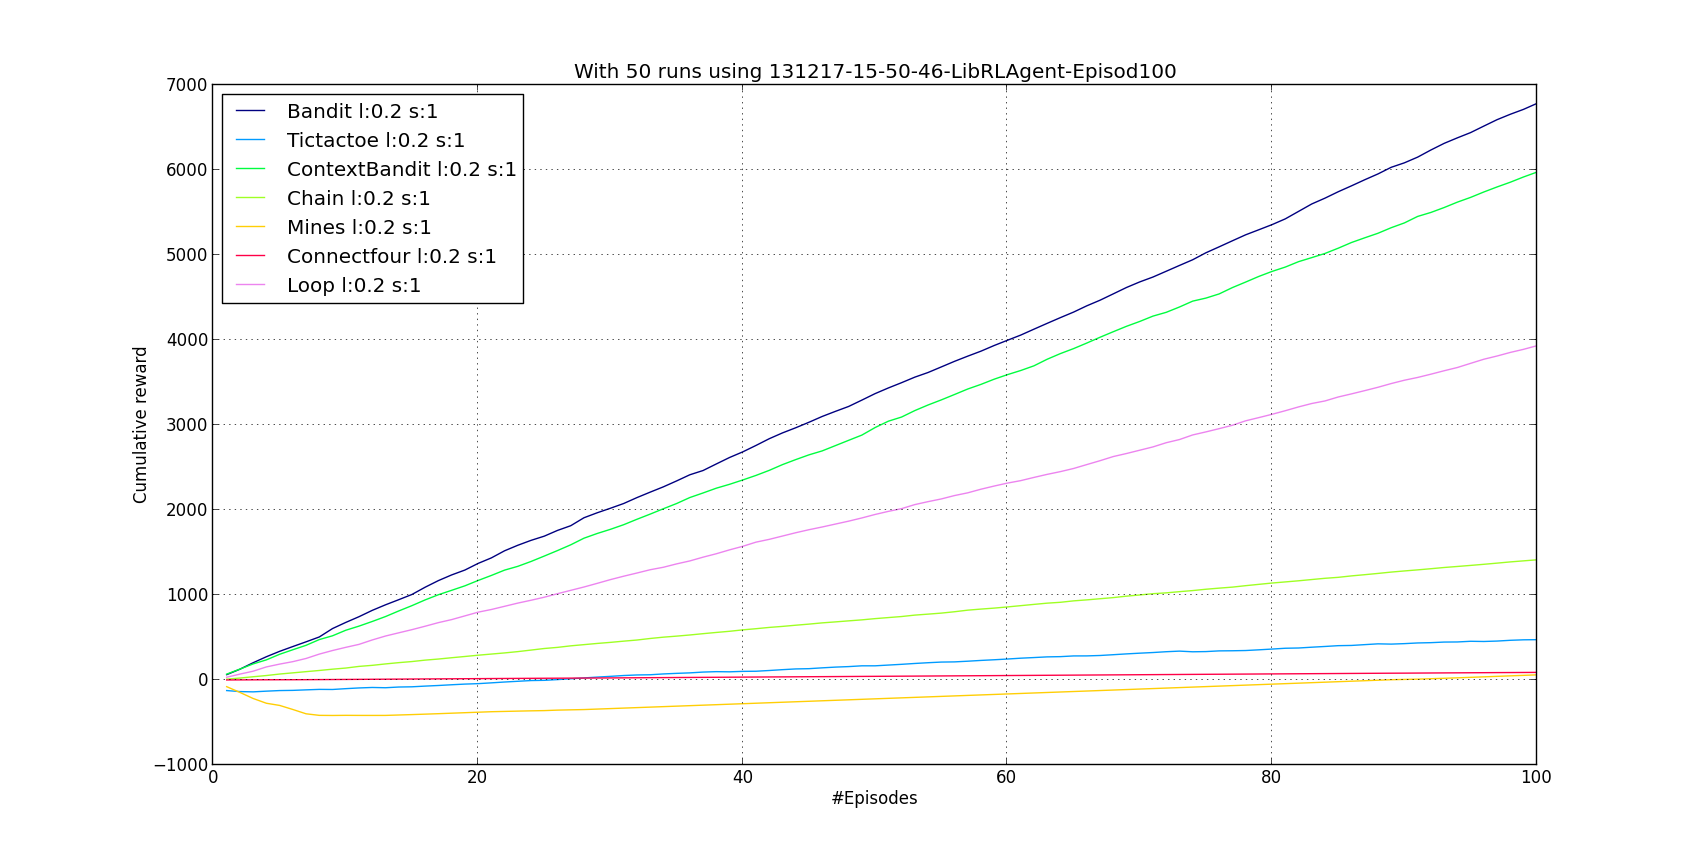
\includegraphics[width=0.5\textwidth]{../data/100episodes_50runs.png}
    \caption{Agents cumulative reward averaged over 50 runs}
    \label{fig:cumreward}
\end{figure}

Sweep $\lambda$
\begin{figure}[h]
    \centering
    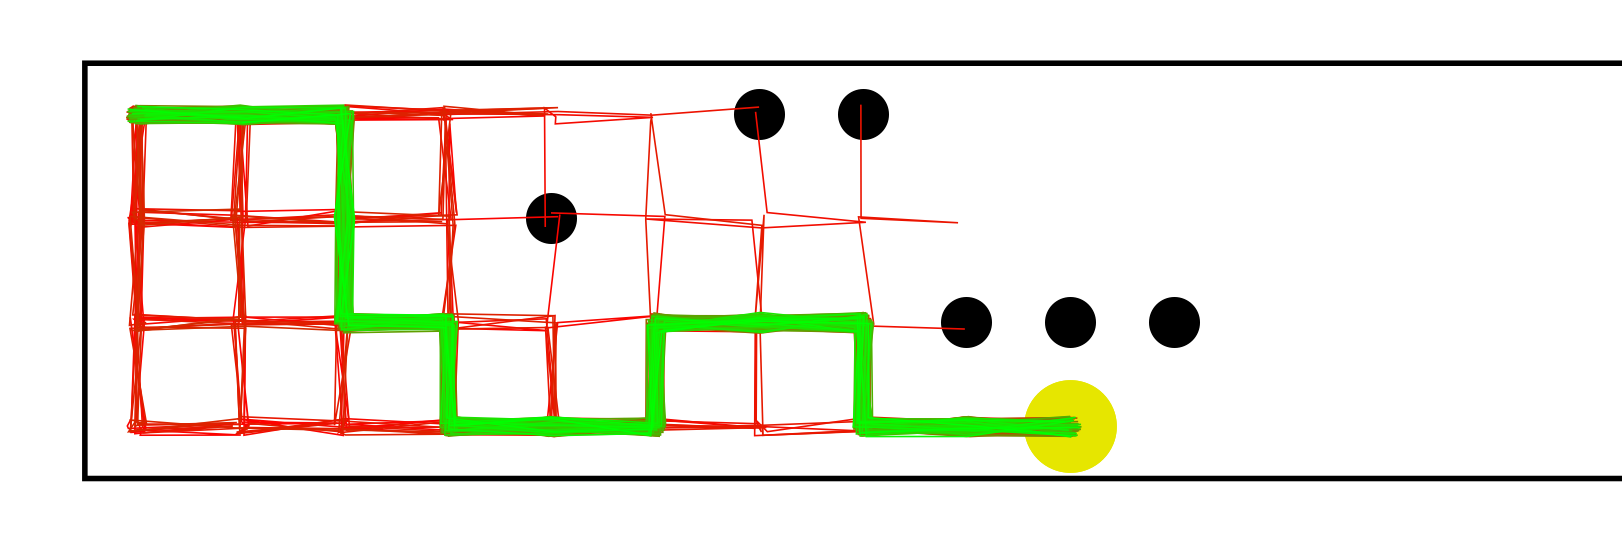
\includegraphics[width=0.5\textwidth]{../data/minPlot.png}
    \caption{Example of how the agent learns a short path from start to goal (yellow). The agent traverse the world 100 times, early attempts are coloured red, later green. Hitting a mine (black) costs a penalty. Every  }
    \label{fig:awesome_image}
\end{figure}

The yellow line indicates the performance on the mines environment and the learning phase of the agent is clear after around 10 episodes. Connect four, red in Fig~\ref{fig:cumreward}, has a much lower maximum reward than the other environments hence it is closer to zero but still increasing.

Training vs the test environments, under the assumption that they are good representation for what we faced in the competition.

All code is found at https://github.com/Oscarlsson/RL-competition
